\documentclass[11pt, oneside,table]{article}   	% use "amsart" instead of "article" for AMSLaTeX format
%\usepackage{geometry}                		% See geometry.pdf to learn the layout options. There are lots.
\usepackage[margin=.9in]{geometry}
\geometry{letterpaper}                   		% ... or a4paper or a5paper or ... 
%\geometry{landscape}                		% Activate for for rotated page geometry
\usepackage[parfill]{parskip}    		% Activate to begin paragraphs with an empty line rather than an indent
\usepackage{graphicx}				% Use pdf, png, jpg, or eps� with pdflatex; use eps in DVI mode
\usepackage{moreverb}						% TeX will automatically convert eps --> pdf in pdflatex		
\usepackage{amssymb}
\usepackage{mathtools}
\usepackage[framed,numbered,]{mcode}
\usepackage{listings}
\usepackage{xcolor}
\usepackage{amsmath}
\usepackage{placeins}
\usepackage{float}
\restylefloat{table}
\lstset { %
    backgroundcolor=\color{black!7}, % set backgroundcolor
    basicstyle=\footnotesize,% basic font setting
}

\newcommand{\bigo}{$\mathcal{O}$}

\title{MATH 6644\\Project 1}
\author{Stephan Boettcher}
%\date{}                                           % Activate to display a given date or no date

\begin{document}
\maketitle
\section*{Part 1}

{\it Discretize the following differential equation:

$$\begin{cases} -u'' =2x-\frac{1}{2}& \ \ x\in [0,1] \\ u(0)=1, & u(1)=-1 \end{cases}
$$
by centered difference scheme with n interior mesh points. Solve the resulting linear system by Conjugate Gradient (CG), Preconditioned CG with Sine transform to construct the preconditioner.}

The one-dimensional equation given above can be solved with numeral method analysis or directly as a function of x. The solved equation then can be used to check the validity of the numerical methods. When solved directly, the equation becomes:
$$u(x) = -0.333333 x^3+0.25 x^2-1.91667 x+1
$$


The discretized one-dimensional equation above was solved by the central difference scheme with $n$ interior points. The resulting problem is then an $(n+2)\times (n+2)$ matrix, A, and $(n+2)\times 1$ vectors, x and b. The problem was solved using both the Conjugate Gradient (CG) method and the Preconditioned CG method with a Sine transform preconditioner, $S$. The $S$ matrix was defined as:

$$[S]_{j,k}=\sqrt{\frac{2}{n+1}}sin\Big(\frac{\pi jk}{n+1}\Big)
$$

The A matrix formed from the discretized equation forms a tridiagonal matrix, with elements directly on the primary diagonal as well as elements one diagonal above and below the primary diagonal. This sparse matrix was then run with the Conjugate Gradient(CG) method. The CG method is one of the most prominent iterative methods for solving sparse matrices as it converges much more quickly than other iterative methods such as steepest descent. The Conjugate Gradient iterates in such a way that each new residual is orthogonal to all the previous residuals and search directions. Each new search direction is constructed is A-orthogonal to all the previous residuals and search directions, thus using the Krylov subspace to iterate more efficiently. The CG method was run with $n$ interior points from 256 to 16384. As the values of $n$ increased, the time necessary to complete the iteration increased proportionally. The final results of the CG method can be found in Figure \ref{p1}.  Figure \ref{final} shows the CG method approaching After the CG method completed, the $S$ matrix, used in the PCG method, was formed. 

%\begin{figure}[!h]
%\begin{center}
%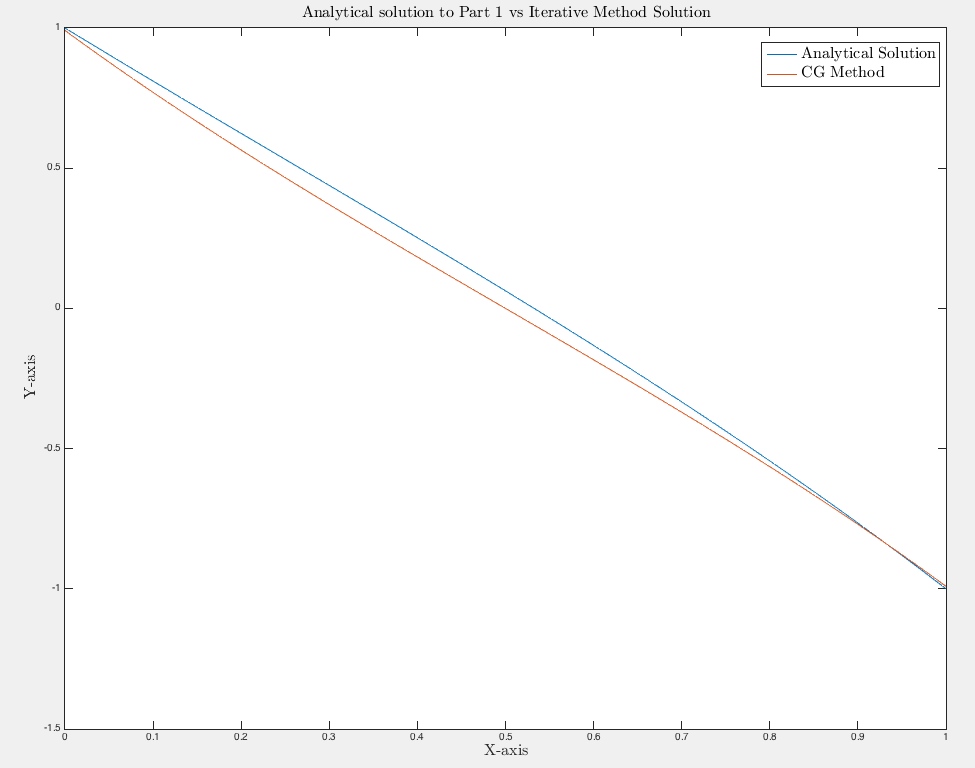
\includegraphics[width=130mm]{p1s.png}
%\caption{Convergence of the CG method.}
%\label{final}
%\end{center}
%\end{figure}

The $S$ matrix was formed in two different ways to determine the most efficient method. The first method was using Matlab's vector math and \mcode{parfor} to form the matrix in parallel. This was achieved with the following code:

\begin{lstlisting}
k=1:runs(a); %generates a vector from 1 to the length of n. 
%runs contains the list of n values and a is the current iteration.
parfor j=1:runs(a)  %Parallel for loop in matlab
        S(j,k)=sqrt(2/(n+1))*sin((pi*j*k)/(n+1)); %form an entire column of values
end
\end{lstlisting}

This code was run with 4 workers in parallel, allowing for a theoretical 4x improvement over the serial code. Figure \ref{parfor} shows the runtime for the parallel code vs serial code.  As is common with parallel code, for small values of $n$, the serial code outperforms the parallel. However, for larger $n$ values, the 4x speedup is achieved. The $S$ matrix then was formed using Matlab's Discrete Sine Transform(DST) command, \mcode{dst(x)}. Figure \ref{parfor} shows the runtime for the built in DST command which proved to be slower than the parallel code. Thus for the remainder of this portion of the project, the parallel code was used. 

\begin{figure}[htbp]
\begin{center}
\begin{tabular}{ | c|c|c| c|}
\hline
  n & Serial (sec) & Parallel For(sec) & DST (sec)\ \\\hline
  258 &0.0194 & 0.0494& 0.5190 \\\hline
  514 &0.0111 & 0.0564 & 0.0196\\\hline
  1026 &0.0423 & 0.0771 & 0.0706\\\hline
  2050 &0.1704 & 0.1439 & 0.2003 \\\hline
  4098 &0.5087 & 0.4694 &1.1024 \\\hline
  8194 &8.1068 & 1.9299 & 3.9583\\\hline
  16386 &37.3268 & 7.9876 & 29.3784\\\hline
  % Design2 &300 & 380 & 370 & 34 & 40& 400& 100& 50& 100& 100 \\\hline
%  Design3 &300 & 600 & 580 & 40 & 50& 550& 100& 150& 200& 250 \\\hline

\end{tabular}
\caption{Runtime for generating the $S$ }
\label{parfor}
\end{center}
\end{figure}



The $S$ matrix acted as a preconditioner to the tridiagonal $A$ matrix. A preconditioned is used to make a problem that is difficult to solve, simpler. The preconditioner is customized and tailored to the problem at hand. For this problem, preconditioning the $A$ matrix by $SAS^T$ results in a diagonal matrix. To achieve extremely fast convergence rates, the preconditioner matrix was split. After preconditioning $A$ with the $S$ matrix, the  inverse, $(SAS^{T})^{-1}$, was calculated and passed to the PCG method. As a result, the PCG method was able to achieve extremely fast convergence rates. While this method does require two matrix-matrix multiplications to setup the preconditioned $A$ matrix, the resulting diagonal matrix was extremely easy to solve. The inverse of the diagonal matrix, $(SAS^{T})^{-1}$, can be calculated in  \bigo(n) time, as the inverse of a diagonal matrix is the inverse of each element on the diagonal. With the chosen preconditioner, each run of the PCG was able to converge in 1 iteration. 


\begin{figure}[htbp]
\begin{center}
\begin{tabular}{ |c|c|c| c|c|}
\hline
  n & CG iterations & CG runtime (sec) & PCG iterations & PCG runtime (sec)\ \\\hline
258 & 129 & 0.023895 & 1 & 0.294494 \\\hline
514 & 257 & 0.014975 & 1 & 0.023645 \\\hline
1026 & 513 & 0.193338 & 1 & 0.111805 \\\hline
2050 & 1025 & 2.468402 & 1 & 0.809114 \\\hline
4098 & 2049 & 18.554962 & 1 & 5.579513 \\\hline
8194 & 4097 & 145.323975 & 1 & 40.182528 \\\hline
16386 & 8193 & 1144.595261 & 1 & 326.499772 \\\hline
  % Design2 &300 & 380 & 370 & 34 & 40& 400& 100& 50& 100& 100 \\\hline
%  Design3 &300 & 600 & 580 & 40 & 50& 550& 100& 150& 200& 250 \\\hline

\end{tabular}
\caption{Runtimes and iteration counts for the CG and PCG methods }
\label{p1}
\end{center}
\end{figure}

As can be seen in Figure \ref{p1}, the PCG method is able to converge in one iteration and in much less time than the CG method. When recording the timing for the PCG method, the time required to form the $S$ matrix was not accounted for, but can be found in Figure \ref{parfor}. The recorded time for the PCG method did account for the two costly matrix multiplication operations, which were undoubtedly the source of much of the runtime. Regardless, the results are impressively conclusive. The PCG method is significantly faster than the regular CG method for this problem. The runtimes for both methods actually decrease for the $n=512$ interior mesh point case ($n=514$ total points). This is actually due to bandwidth/latency optimizations that are occurring at the processor/memory cache level. As n increases, the number of CG iterations also roughly doubles. However, for both the CG and the PCG method, the time to complete the method increase by a factor of 8. The primary driver of this increase is the matrix multiplication that occurs in each method. 





\section*{Part 2}
{\it Perform the CG and PCG for Toeplitz systems using both Strang's and Chan's circulant matrices as the preconditioners.} \newline


The a matrix is defined as a Toeplitz matrix if it has the following form: 
$$
A = \begin{bmatrix}
a_0& a_{-1}& \dots & a_{2-n}    & a_{1-n}      \\[0.3em]
a_1& a_{0}&  a_{-1} & a_{2-n}    & a_{1-n}      \\[0.3em]
\vdots& a_{1}& a_0 & \ddots   & \vdots     \\[0.3em]
a_{n-2}&  & \ddots & \ddots   & a_{-1}      \\[0.3em]
a_{n-1}& a_{n-2}& \dots & a_1    & a_{0}      \\[0.3em]
     \end{bmatrix}
  $$
  
  Toeplitz matrices are extremely useful and arise in solutions to differential and integral equations, as well as applications such as signal processing and optical analysis. A common special case of Toeplitz matrices are {\it circulant} matrices. A matrix is called circulant if it has the form of: 
  
  $$
C = \begin{bmatrix}
c_0& c_{-1}& \dots & c_{-(n-2)}    & c_{-(n-1)}      \\[0.3em]
c_{-(n-1)}& c_{0}&  c_{-1} &  \dots   &       \\[0.3em]
c_{-(n-2)}& c_{-(n-1)}& c_0 &    & \vdots     \\[0.3em]
   \vdots &  & & \ddots   &       \\[0.3em]
c_{-1}& c_{-2}& \dots &  c_{-(n-1)}    & c_{0}      \\[0.3em]
     \end{bmatrix}
  $$
  
  These circulant matrices approximate and explain the behavior of Toeplitz matrices and thus are useful as preconditioners for the Preconditioned Conjugate Gradient (PCG) method. In order to understand the properties of circulant matrices, one must look at how their eigenvectors are created\cite{toeplitz}\cite{chanAndStrang}\cite{Chan}. The eigenvalues, $\lambda_k$, and eigenvectors, $\nu_k$  are given by $C_n\nu =\lambda \nu$. This can also be expressed as the $n$ difference equations:
  $$ \sum\limits_{k=0}^{m-1} c_{n-m+k}\nu_k+\sum\limits_{k=m}^{n-1}c_{k}\nu_{k-(n-m)} =\lambda\nu_m \ \ \ \ \ \  m=0:n-1
  $$
  
  The above can be solved easily and since it is a linear equation with constant coefficients, $\nu_k$ can be replaced with $\nu_k=\rho^k$. This is analogous to $y(t)=e^{st}$ in time invariant differential equations. Substituting in $\rho$ and canceling terms yields:
    $$ \sum\limits_{k=0}^{n-1-m} c_{k}\rho^k+\rho^{-n}\sum\limits_{k=n-m}^{n-1}c_{k}\rho^k =\lambda
  $$
  
We can see that by choosing values for rho,  the corresponding eigenvectors will fall out. If we choose $\rho=e^{\frac{-2\pi imk}{n}}$, the eigenvector that comes about is:

$$\nu_m=\frac{1}{\sqrt{n}}\Big(1,e^{\frac{-2\pi im}{n}},\dots,e^{\frac{-2\pi im(n-1)}{n}}\Big)
$$

The curious thing about this particular value set for $\rho$ is that this is the discrete Fourier Transform (DFT) of the sequence $c_k$. Thus, we can actually recover $c_k$ by taking the inverse DFT of the eigenvalues, $\lambda_k$. Since the circulant matrix is made up of one row of values that have been shifted right as a function of their row number, the eigenvalues of $C_n$ can be found by merely taking the DFT of the first column of $C_n$. This allows one to diagonalize a circulant matrix by the Fourier matrix, $F_n$:
  
  $$ C_n =F_n^*\Lambda_nF_n
  $$
  where $[F]_{j,k}=\frac{1}{\sqrt{n}}e^{\frac{2\pi ijk}{n}}$ for $0\le j,k\le n-1$ and $\Lambda$ is a diagonal matrix holding the eigenvalues of $C_n$. The DFT operation is extremely efficient(\bigo($n\ log\ n$)) compared to traditional matrix-vector multiplication(\bigo($n^2$) at best). Once $\Lambda$ has been obtained, the products $C_v\vec{y}$ and $C_n^{-1}\vec{y}$ can be computed in \bigo($n\ log\ n$).
  
 
 Circulant matrices can be used to speed up the Conjugate Gradient (CG) method, when solving a symmetric positive definite Toeplitz system:
 $$A_n\vec{x}=\vec{b}
 $$
 Two commonly used circulant preconditioners for speeding up the CG method are G. Strang's\cite{strang} circulant preconditioner and T. Chan's\cite{Chan} circulant preconditioner. String's conditioner is defined by the rules:
 
 
 $$\begin{cases} a_j & 0\le j \le [\frac{n}{2}] \\
a_{j-n} & [\frac{n}{2} < j < n 
c_{n+j} 0<-j <n
 \end{cases}
$$
Where $[\ \cdot\ ]$ is the \mcode{floor()} algorithm. For a symmetric $4\times4$ matrix, this would look like:

   $$
C_{strang} = \begin{bmatrix}
c_0& c_{1}& c_{2} & c_{1}    \\[0.3em]
c_{1}& c_{0}&  c_{1} &  c_2      \\[0.3em]
c_{2}& c_{1}& c_0 &   c_1     \\[0.3em]
c_{1}& c_{2} &  c_{1}    & c_{0}      \\[0.3em]
     \end{bmatrix}
  $$
  
The diagonals containing the value $c_1$  appear in the two corners, where as the $A$ matrix had new, and possibly smaller, values $a_{n-1}$. In the Strang circulant, this information is left out. In order to precondition the $A$ matrix, the  inverse of Strang circulant must be applied to the $A$ matrix. Inverting the Strang circulant is done with the following code:
\begin{lstlisting}
a1=ifft(fft(Cn(:,1)).^-1)'; %DFT first column of Cn, then invert, then iDFT
a1s=zeros(length(a1));
     parfor j=1:length(A)
            a1s(:,j)=circshift(a1,j-1,2); %Matlab's circular shifting algorithm
     end
\end{lstlisting}
 
 where $C_n$ is the circulant, \mcode{fft} is the Fast Fourier Transform (FFT), and \mcode{ifft} is the inverse FFT. The Chan preconditioner is created in a similar manner. 
 
 The Chan circulant is defined as:
 
 $$\begin{cases} 
\ \frac{(n-j)a_j+ja_{j-n}}{n}& 0\le j \le n \\
\ a_{j-n} & \frac{n}{2} < j < n 

 \end{cases}
$$

which for a symmetric $4\times4$ matrix would look like:

   $$
C_{strang} = \begin{bmatrix}
c_0& \alpha& c_{2} &\alpha   \\[0.3em]
\alpha& c_{0}&  \alpha&  c_2      \\[0.3em]
c_{2}& \alpha& c_0 &   \alpha   \\[0.3em]
\alpha& c_{2} &  \alpha  & c_{0}      \\[0.3em]
     \end{bmatrix}
  $$

 where $\alpha=\frac{3a_1+a_3}{4}$. For larger matrices the value of $\alpha$ will change to follow the above set of rules. Unlike the Strang circulant, the information from $a_3$ is not lost, but is incorporated in via the $\alpha$ term. This is important as it allows this particular circulant to better mimic the original $A$ matrix. This averaging term allows the spectrum of $C^{-1}A$ to lie completely within that of the Strang circulant and hence have a smaller condition number. 
 
 As the Chan circulant has the same eigenvalue properties as the Strang circulant, it can be inverted using the same code as presented above. Once inverted, the circulant can then be passed to the Preconditioned Conjugate Gradient method for processing. 
 
 The Preconditioned Conjugate Gradient method is nearly identical to the Conjugate Gradient method. In fact, they share ~95\% of the same code. The only real difference is in the preconditioner that is applied to the matrix $A$ and the creation and use of a $z$ parameter. The PCG method utilizes the stability of the CG method and  attempts to further speed it up with a preconditioner. The role of the preconditioner in this process is to reduce the condition number of the problem so that it may be solved more readily. Iterative methods such as the PCG and CG methods are most suited for use with sparse matrices. If $A$ is dense, it may be more worthwhile to attempt gaussian elimination, unless a proper preconditioner can be found. If a preconditioner, $C$ can be found that diagonalizes the dense matrix $A$ then the much faster PCG method can be employed. 
 
 For this project, both the Strang ($C_s$) and the Chan ($C_c$) circulant matrices were used to condition two different $A$ matrices. The solution to $A\vec{x}=\vec{b}$ was then solved with the CG and PCG method and the results were compared. The first symmetric Toeplitz system solved was defined as:
 
$$a_k=|k+1|^{-p} \ \ \ \ \ p=2,1,\frac{1}{10},\frac{1}{100}
$$ 
 
 where $a_k$ is the lower triangular portion of $A_n$. Each $A$ matrix generated for this case was tested to see if it maintained its symmetric positive definite (SPD) characteristics. This was done by checking the eigenvalues of the system for each $p$ value. Even for $p\le1$, this system did remain SPD. 
 
 For each value of $p$, an $n\times n$ $A$ was generated, where the value of $n$ were set to $n=50$, $100$, $200$, $400$, $800$, $3200$, $6400$. Thus, for each value of $p$, 8 different $A$ matrices were solved, generating a total of 32 solutions per iterative method tested. The value of $\vec{b}$ for these systems was generated by a random number generator and changed for each iteration.  To evaluate the performance of each iterative method, the wall clock time required to solve the system of equations was evaluated. Unfortunately, Matlab is unable to easily collect FLOPS statistics for a given time and wall clock time was required to be used for comparison. The CG method was used as a baseline to compare PCG method with the Strang preconditioner and the Chan preconditioner. The results for the CG method are interleaved into the  results for the two PCG methods, for easy of comparison. The PCG method using the Strang preconditioner is found in Figures \ref{sp2}, \ref{sp1}, \ref{sp01}, and \ref{sp001}. The PCG method used the inverse of the Strang preconditioner, $C_s^{-1}$, as the actual preconditioning matrix for this problem. Using the inverse of the $C_s$ matrix results in drastically faster convergence rates for the PCG method. 
 
\begin{figure}[htbp]
\begin{center}
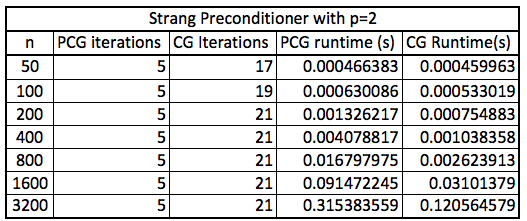
\includegraphics[width=125mm]{sp2.png}
\caption{The results of the CG iterative method and the PCG iterative method with a Strang circulant preconditioner and p=2}
\label{sp2}
\end{center}
\end{figure}
\begin{figure}[htbp]
\begin{center}
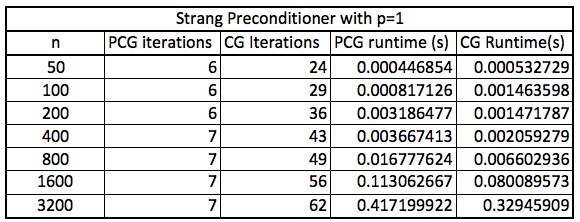
\includegraphics[width=125mm]{sp1.png}
\caption{The results of the CG iterative method and the PCG iterative method with a Strang circulant preconditioner and p=1}
\label{sp1}
\end{center}
\end{figure}

As can be seen in Figures \ref{sp2} and \ref{sp1}, for small values of $n$, and for the better conditioned matrices ($p=2$,$p=1$) the CG method is actually marginally more efficient then the PCG method, when looking at runtimes. However, when comparing the PCG number of iteration necessary to converge, the numbers are somewhat striking. The number of iterations required to converge for the PCG method was significantly less than the CG method. As the $p$ value used in the creation of the $A$ matrix decreases, the CG method rapidly loses its advantage and the PCG method becomes more efficient. Figures \ref{sp01} and \ref{sp001} show how the number of iterations required for the CG method to converge increases. Unlike the CG method, with the Strang preconditioner, the PCG method remains quite stable in the number of iterations required.  This stability allows for the runtimes of the method to also remain small. 

\begin{figure}[htbp]
\begin{center}
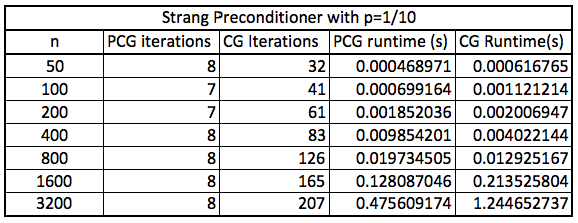
\includegraphics[width=125mm]{sp01.png}
\caption{The results of the CG iterative method and the PCG iterative method with a Strang circulant preconditioner and p=$\frac{1}{10}$}
\label{sp01}
\end{center}
\end{figure}
\begin{figure}[htbp]
\begin{center}
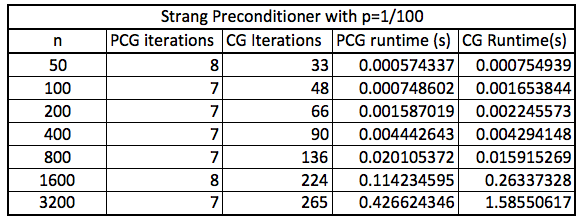
\includegraphics[width=125mm]{sp001.png}
\caption{The results of the CG iterative method and the PCG iterative method with a Strang circulant preconditioner and p=$\frac{1}{100}$}
\label{sp001}
\end{center}
\end{figure}

 By analyzing the runtimes of the PCG method over the various runs and with multiple $p$ values, an overall growth rate of the runtimes can be determined. Ideally, the PCG method runtimes grow at a rate of \bigo($n\, log\, n$). For many runs, the growth pattern was \bigo($3n\, log\, n) \ge$ \bigo($x$) $\ge$ \bigo$(\frac{1}{2}\, n\, log\, n$) $\approx$ \bigo($n\, log\, n$) where $x$ is the growth rate for a given subset of runs. Since the number of iterations remained fairly constant, calculating these qualities becomes much more straight forward. Thus, the PCG method with the Strang circulant achieved a good speedup over the traditional CG method when the $A$ matrix became less friendly. 


\begin{figure}[htbp]
\begin{center}
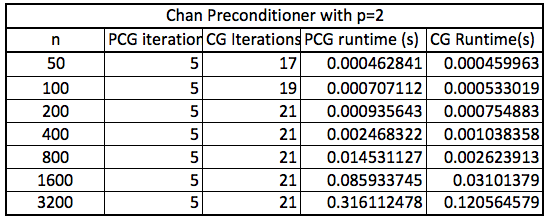
\includegraphics[width=125mm]{cp2.png}
\caption{The results of the CG iterative method and the PCG iterative method with Chan's circulant preconditioner and p=2}
\label{cp2}
\end{center}
\end{figure}
\begin{figure}[htbp]
\begin{center}
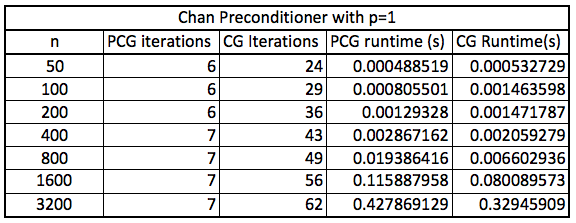
\includegraphics[width=125mm]{cp1.png}
\caption{The results of the CG iterative method and the PCG iterative method with  Chan's  circulant preconditioner and p=1}
\label{cp1}
\end{center}
\end{figure}

The PCG method utilizing the Chan preconditioner is found in Figures \ref{cp2}, \ref{cp1}, \ref{cp01}, and \ref{cp001}. As can be seen in the two Figures, the PCG method is faster than the CG method. Close analysis of the use of Chan's preconditioner vs Strang's preconditioner reveals that both methods are roughly equivalent. The runtimes for both methods are nearly identical for the two preconditions, as are the number of iterations required to converge.  As stated before, the structure of the Chan preconditioner allows it to be in the subspace of the Strang preconditioner and thus has a better condition number. This theoretically allows for a faster convergence of the iterative method. However, for the problem size and complexity of this project, the two methods were roughly equivalent. 

\begin{figure}[htbp]
\begin{center}
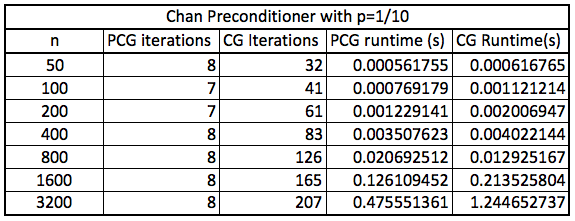
\includegraphics[width=120mm]{cp01.png}
\caption{The results of the CG iterative method and the PCG iterative method with Chan's circulant preconditioner and p=$\frac{1}{10}$}
\label{cp01}
\end{center}
\end{figure}
\begin{figure}[htbp]
\begin{center}
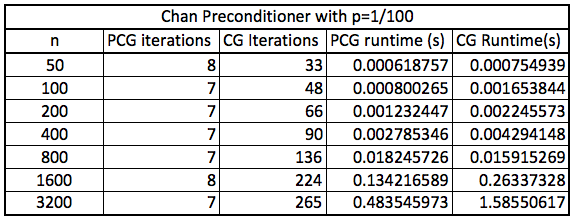
\includegraphics[width=120mm]{cp001.png}
\caption{The results of the CG iterative method and the PCG iterative method with Chan's circulant preconditioner and p=$\frac{1}{100}$}
\label{cp001}
\end{center}
\end{figure}


 
 \FloatBarrier
 
 
The second symmetric Toeplitz system is defined by:

$$ a_k=\frac{1}{2\pi}\int\limits^\pi_{-\pi}f(\theta)e^{-ik\theta}d\theta,\ \ \ \ \ k=0,\pm 1, \pm2, \dots,
$$
where $f(\theta)=\theta^4 +1$ for $-\pi\le\theta\le\pi$. This means that $a_k$ is the Fourier coefficients of $f(\theta)$ and were computed via FFT. For the second system, the PCG and CG method were each run for the 6 different values of $n$ only. Once again, the CG method was compared to the PCG method with Chan's preconditioner and Strang's preconditioner. For this new $A$ matrix based upon the Fourier coefficients of

 
 \begin{figure}[htbp]
\begin{center}
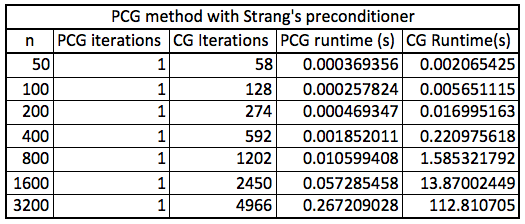
\includegraphics[width=120mm]{pcsb.png}
\caption{The final runtimes of the CG iterative method and the PCG iterative method with a Strang circulant preconditioner.}
\label{pcgB1}
\end{center}
\end{figure}

\begin{figure}[htbp]
\begin{center}
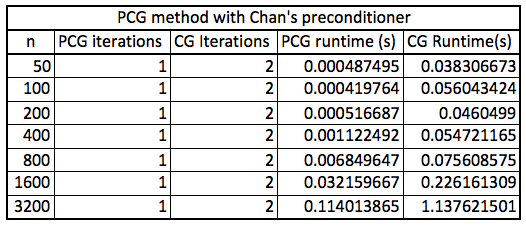
\includegraphics[width=120mm]{pccb.png}
\caption{The final runtimes of the CG iterative method and the PCG iterative method with a Chan circulant preconditioner.}
\label{pcgB2}
\end{center}
\end{figure}
 
 

 
% \begin{table}[H!]                                
%\centering                                       
%\begin{tabular}{|c|c|c|c|c|c|}                     
%\hline        
%Method & n & P= 2 & P=1 & P=$\frac{1}{10}$ &P=$\frac{1}{100}$ \\ \hline                              
%CG	&50		&0.1087 & 0.0951 & 0.1114 & 0.0771 \\    \hline                                           
%PCG&50		&0.1312 & 0.2258 & 0.2089 & 0.2173 \\   \hline                                           
%CG	&100		&0.1162 & 0.1216 & 0.1031 & 0.0774\\    \hline                                           
%PCG&100		&0.1447 & 0.1335 & 0.1238 & 0.1221 \\   \hline                                           
%CG	&200		&0.1170 & 0.1233 & 0.1035 & 0.0798 \\    \hline                                           
%PCG	&200		&0.1340 & 0.1470 & 0.1352 & 0.1213 \\   \hline                                           
%CG	&400		&0.1068 & 0.1226 & 0.1405 & 0.0862 \\    \hline                                           
%PCG	&400		&0.1312 & 0.1412 & 0.1560 & 0.1188   \\   \hline                                           
%CG	&800		&0.1199 & 0.1055 & 0.1193 & 0.0950  \\    \hline                                           
%PCG	&800		&0.1314 & 0.1544 & 0.1715 & 0.1415 \\   \hline                                           
%CG	&1600	&0.1367 & 0.1929 & 0.3449 & 0.3500 \\    \hline                                           
%PCG	&1600	&0.2624 & 0.2854 & 0.2847 & 0.2674  \\   \hline                                           
%CG	&3200	&0.2270 & 0.4816 & 1.5152 & 1.5503  \\    \hline                                           
%PCG	&3200	&0.6958 & 0.8076 & 0.8305 & 0.8286  \\   \hline                                           
%CG	&6400	&0.5824 & 1.6288 & 8.0961 & 8.3655  \\     \hline                                           
%PCG	&6400	&2.6096 & 3.1675 & 3.9813 & 3.3763\\    \hline                                           
%CG	&12800	&2.1291 & 6.3133 & 35.2401 & 52.8248 \\  \hline                                           
%PCG	&12800	&9.2799 & 11.9010 & 14.2468 & 12.6440  \\ \hline                                           
%\end{tabular}                                    
%\caption{MyTableCaption}                         
%\label{table:MyTableLabel}                       
%\end{table}       
 
 \FloatBarrier
\newpage
\begin{thebibliography}{9}
\bibitem{Painless}
J. Shewchuk,
  \emph{An Introduction to the Conjugate Gradient Method Without the Agonizing Pain}.
  Carnegie Mellon University
  1994.

\bibitem{toeplitz}
R. Gray, 
  \emph{Toeplitz and Circulant Matrices: A review}.
 Stanford University
  2006.

\bibitem{strang}
G. Strang,
  \emph{A Proposal for Toeplitz Matrix Calculations}.
  Stud. Appl. Math., 74(1986), pp171-176.
  
  \bibitem{chanAndStrang}
R. Chan and G. Strang,
  \emph{Toeplitz Equations by Conjugate Gradients with Circulant Preconditioner}.
   SIAM J. Sci. Stat. Comput., 10(1989), pp 104-117.
  
  \bibitem{Chan}
T. Chan,  
  \emph{An Optimal Circulant Preconditioner for Toeplitz Systems}.
SIAM J. Sci. Stat. Comput. 9
(1988) pp 766-771.
\end{thebibliography}



%\begin{figure}[htbp]
%\begin{center}
%\begin{tabular}{ | l | c|c| c| c | c | c| c| c| c  | c | }
%\hline
%  &A & B & C &D &E&F&G&H&I&J\ \\\hline
%  Design1 &240 & 350 & 305 & 30 & 35& 400& 90& 0& 30& 300 \\\hline
%% Design2 &300 & 380 & 370 & 34 & 40& 400& 100& 50& 100& 100 \\\hline
%%  Design3 &300 & 600 & 580 & 40 & 50& 550& 100& 150& 200& 250 \\\hline
%
%\end{tabular}
%\caption{Design 1 Parameters}
%\end{center}
%\end{figure}
%
%The isometric view of this design can be seen in Figure \ref{d1i}. The large cylinder was plotted using multiple instances of the \mcode{surf} command on two cylinders. Figure \ref{d1y} and Figure \ref{d1z} show the printer design in the X-Y and X-Z plains, respectively.
%
%\begin{figure}[htbp]
%\begin{center}
%\includegraphics[width=160mm]{d1iso.png}
%\caption{An isometric view of Design 1}
%\label{d1i}
%\end{center}
%\end{figure}



\end{document}  